% !TEX root = mythesis.tex

%==============================================================================
\chapter{Signal Extraction and Background Processes}
\label{sec:tZq}
%==============================================================================
The chapter provides a detailed description about the \tZq process and its trilepton decay channel
which is the signal in this analysis. The baseline event selection defined to extract maximum signal is
given in \cref{sec:evsel}. The different background processes are described in
\cref{sec:bkg}. In addition, information about Monte Carlo simulated samples for signal and 
background processes can be found in \cref{sec:MCinfo}. The various sources of systematic uncertainties
are outlined in \cref{sec:systinfo}. Moreover, a brief explanation of neural networks is also provided 
at the end. 
\section{The \tZqsec production}
\label{sec:tZqdescribe}
Since at the LHC, high energies are attainable by particles, production of heavy particles such as the
\Ptop-quark and its related processes, become highly probable. For this reason, LHC is called a top 
factory. One of the
rare processes at the LHC is the associated production of the \Ptop-quark and the 
\PZ-boson through electroweak interactions. It is referred to as the \tZq production. Its LO $t$-channel
Feynman diagrams are shown in \cref{fig:tZqfeyn}. A \PZ-boson is radiated from any one of the incoming or outgoing 
quarks (\cref{fig:tZqfeyna}) or from the exchanged \PW-boson (\cref{fig:tZqfeynb}). In addition to these
resonant contributions, there is also a small non-resonant contribution 
in the form of $tl^+l^-q$ (\cref{fig:tZqfeync}) which is also accounted for in this analysis. 
The associated \Ptop-quark is produced through interactions such as $\Pup+\Pbottom \rightarrow \Pdown+\PZ+\Ptop$ or 
$\APup+\Pbottom \rightarrow \APdown+\PZ+\Ptop$ whereas \APtop-quark is produced 
via the charge conjugate processes. 

% The NLO QCD
% corrections for \tZq are small and therefore any possible deviations from the SM can be 
% studied in the context of SM Effective Field Theory. 


\begin{figure}[htbp]
    \centering
    % \begin{subfigure}{0.35\figwidth}
    %   \centering
    %      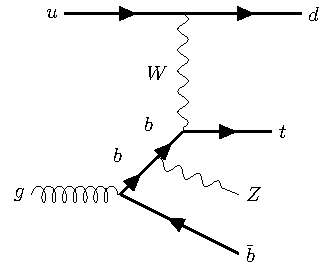
\includegraphics[width=\textwidth]{tZq_Zfromb.pdf}
    %      \caption{}
    %      \label{fig:tZqfeyna}
    % \end{subfigure}
    % \qquad
    \begin{subfigure}{0.35\figwidth}
      \centering
      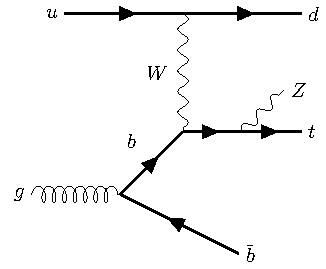
\includegraphics[width=\textwidth]{tZq_Zfromtop.pdf}
      \caption{}
      \label{fig:tZqfeyna}
    \end{subfigure}
    \begin{subfigure}{0.35\figwidth}
      \centering
      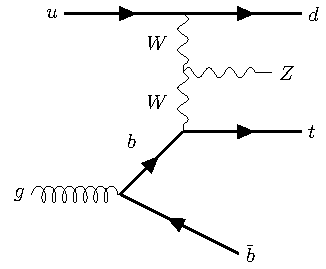
\includegraphics[width=\textwidth]{tZq_ZfromWW.pdf}
      \caption{}
      \label{fig:tZqfeynb}
    \end{subfigure}
  
  
  \medskip
  
  
  \begin{subfigure}{0.35\figwidth}
      \centering
      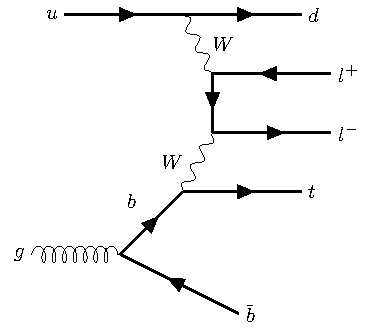
\includegraphics[width=\textwidth]{tZq_nonres.pdf}
      \caption{}
         \label{fig:tZqfeync}
    \end{subfigure}
    % \begin{subfigure}{0.35\figwidth}
    %   \centering
    %   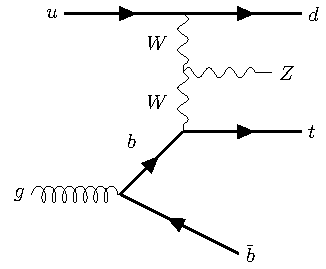
\includegraphics[width=\textwidth]{tZq_ZfromWW.pdf}
    %   \caption{}
    %      \label{fig:tZqfeyne}
    % \end{subfigure}
    % \begin{subfigure}{0.35\figwidth}
    %     \centering
    %     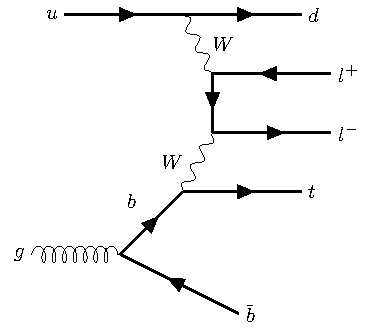
\includegraphics[width=\textwidth]{tZq_nonres.pdf}
    %     \caption{}
    %      \label{fig:tZqfeynf}
    %   \end{subfigure}
  
  \caption[Feynman diagrams at LO for the \tZq-production]{Feynman diagrams at 
  LO for the \tZq-production. The \PZ is radiated either from one of the
  quarks or from the exchanged W boson. }
  \label{fig:tZqfeyn}
  \end{figure}

The \tZq production is interesting to study because it probes the coupling of \Ptop and \PZ as well as 
the $\PW\PW\PZ$ coupling. In other words, it allows the coupling
of two bosons and the coupling of a fermion to a boson to be studied in a single interaction. Moreover, 
it can provide a solid basis to study similar processes such as the $tHq$ process. 
The theoretical cross-section based on SM prediction is calculated at NLO in QCD
for a dilepton mass more than $\qty{30}{\GeV}$, is $\qtypmerr{102}{5}{2}{\femto\barn}$. The \tZq
process was observed by ATLAS and CMS during the Run-2 of the LHC.
The cross-section, measured by the ATLAS collaboration, is $\qtyerrs{97}{13}{7}{\femto\barn}$~\cite{TOPQ-2018-01} which
is consistent with the SM expectation. 

In order to study this process, one has to note 
that the particles involved are quite heavy and therefore,
the only way to spot them is from their reconstructed decay products. Moreover, depending on the 
branching ratio, there can be several sets of final states.
A common practice is to divide the possible final states into \textit{channels}
based on certain combinations of leptons and jets. This analysis focuses on
the so-called trilepton channel which is described below.

\section{The \tZqsec Trilepton Channel}
As the name suggests, the trilepton decay channel of the \tZq production 
contains final states with three charged leptons, as shown in \cref{fig:tZqtrilep}. The
\Ptop-quark decays almost exclusively into \Pbottom\PW and the corresponding \PW can decay either
leptonically or hadronically. Approximately in 25\% events, \PW decays into a charged lepton and
an associated neutrino. The \PZ-boson can decay either into a pair of leptons or into neutrinos (invisible)
or into hadrons. In approximately 8\% of the produced events, the \PZ boson decays 
into opposite sign same flavour lepton pairs. Its probability 
is equal across the three lepton families (\Pelectron,\Pmuon,\Ptauon) owing to 
lepton flavour universality. It is one of the principles of the SM that the interactions of weak gauge 
bosons and leptons is the same for all the lepton flavours. This analysis includes \PZ decays resulting into electrons or muons 
(\Pelectron\APelectron or \Pmuon\APmuon). The tau leptons are considered if they decay into lighter
leptons (i.e. \Pelectron or \Pmuon). 

\begin{figure}
  \centering
      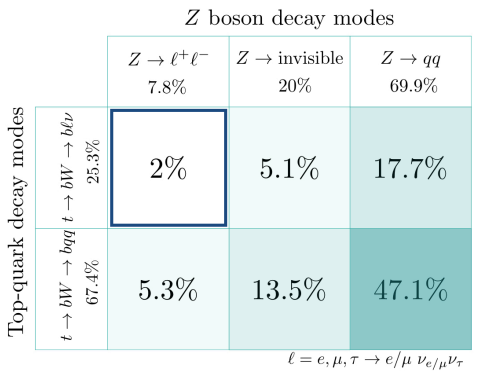
\includegraphics[width=0.6\textwidth]{tZ_decays.png}
      \caption{Branching ratios of possible decays of \Ptop and \PZ, along with the fractions representing
      combination of decays~\cite{irina:2018}}
         \label{fig:tZqdecays}
\end{figure}

The branching fractions of the various possible decays of \Ptop and \PZ is shown in \cref{fig:tZqdecays}.
The combination of both \Ptop and \PZ decaying into leptons occurs in only 2\% of the produced \tZq events.
However, selecting the trilepton decay state has its advantages. First and foremost, the efficiency of 
reconstructing leptons is higher than that of hadrons because of the clean signatures of leptons. 
In addition, a decay state with three leptons is difficult to replicate by 
background processes which ensures signal purity. 
Due to these reasons, the trilepton channel is chosen for studying the 
\tZq process. From this point onward, this will be referred to as the signal.

\begin{figure}
  \centering
      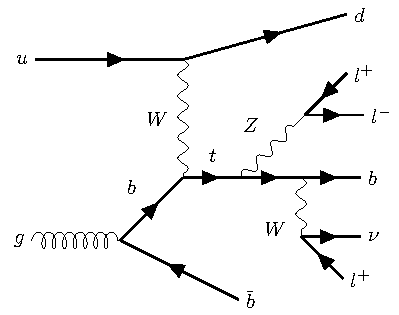
\includegraphics[width=0.45\textwidth]{tZq_Zfromtop_decay.pdf}
      \caption{The \tZq trilepton final state}
         \label{fig:tZqtrilep}
\end{figure}

The accurate reconstruction of \Ptop and \PZ is essential for the efficient identification of signal. 
The \PZ boson is reconstructed from Opposite Sign Same Flavour (OSSF) lepton pair. If all three
leptons have same flavour, the leptons having invariant mass closest to the mass of \PZ, are chosen
for \PZ reconstruction. 

The lepton failing the criteria for \PZ reconstruction is used to reconstruct the \PW boson along with
missing transverse energy. Finally, the \Ptop quark is reconstructed from the \PW and the \Pbottom-tagged
jet having the maximum \pT.

Due to the \Ptop-channel production, one or more jets are produced close to the beam direction. The
forward-jet is defined as the non \Pbottom-tagged jet yielding the maximum invariant mass with the 
leading \Pbottom-jet.

\subsection{Event Selection}
\label{sec:evsel}
In LHC physics, the outcome of a collision between two incoming particles is called as an "event".
An important step in an analysis is to reconstruct the final state of interest from the detector data or in other words, find
possible occurrences of this final state within the collision events. In order to achieve that,
certain requirements are defined in favour of the signal events. The collection of these requirements
is called event selection. For this analysis, the primary event selection is discussed below and
summarised in \cref{tab:selection:srcr}.

\begin{itemize}
  \item \textbf{Leptons}
    \begin{itemize}
      \item Exactly three leptons (\Pelectron or \Pmu), 
      \Ptau is considered if it decays into leptons. These leptons are 
      sorted by their \pT which is required to be at least 27,15 and 10 GeV, respectively.
      
      \item At least 1 OSSF lepton pair with a minimum
      difference between its invariant mass ($m_{ll}$) and $m_Z$. This is to identify 
      which out of the selected leptons originate from \PZ.

      \item A cut on minimum accepted invariant mass, in order to suppress backgrounds 
      not containing a \PZ.

      \item A cut on the transverse mass of the \PW-boson is applied to account for the missing
      transverse energy. 
  \end{itemize}
  \item \textbf{Jets}
  \begin{itemize}
    \item Number of jets are required to be between 2 and 5, with \pT more than \qty{25}{GeV}
    and $|\eta|$ more than 4.5.
    \item Number of \Pbottom-jets are required to be 1 or 2, reconstructed at $85\%$ working 
    point with $|\eta|$ more than 2.5. Events with 2 jets, both \Pbottom-tagged are not considered.
  \end{itemize}


\end{itemize}

\begin{table}[!htbp]
    \footnotesize
    \caption{Event selection}
    \label{tab:selection:srcr}
    \renewcommand{\arraystretch}{1.3}
    \centering
    \begin{tabular}{lccc}
        \toprule
        Variable & \multicolumn{3}{c}{Preselection}\\
        \midrule
        $N_\ell~\left(\ell=e,\mu\right)$ & \multicolumn{3}{c}{$=3$}\\
        & \multicolumn{3}{c}{$\ge 1$ OSSF lepton pair}\\
        $\pT\left(\ell_1,\ell_2,\ell_3\right)$ & \multicolumn{3}{c}{$>$ 27,~15, \qty{10}{\GeV}}\\
        $\min(m_{\ell\ell})$ & \multicolumn{3}{c}{$>$ \qty{20}{\GeV}} \\
        $|m_{\ell\ell} - m_{Z}|$ & \multicolumn{3}{c}{$<$ \qty{10}{\GeV}} \\
        \mtw & \multicolumn{3}{c}{$>$ \qty{30}{\GeV}} \\
        $N_\text{jets}\left(\pT>25~\mathrm{GeV}\right)$ & \multicolumn{3}{c}{2-5} \\
        $N_{b-\text{jets}} @ 85\%$ & \multicolumn{3}{c}{1-2 (no $2j2b$)} \\
        % & SR & \CRttZ & \CRVV \\
        % $N_\text{jets}\left(\pT>25~\mathrm{GeV}\right)$ & 2-5 & $\ge 6$ & 2-5 \\
        % $N_{b-\text{jets}} @ 85\%$ & 1-2 (no $2j2b$) & $\ge 1$ & 0 \\
        \bottomrule
    \end{tabular}
    \end{table}


It is important to note here that these requirements are chosen to 
maximise the probability of selecting signal events
but in reality there are background processes that mimic the \tZq signature
and therefore, contaminate the selected signal events. 

\section{Background processes}
\label{sec:bkg}

The background processes for \tZq process can be classified according to the number of prompt (or real)
leptons in the final state. A lepton is labelled prompt if it originates from either a \Ptau or a 
massive boson. On the other hand, non-prompt or fake leptons are objects misidentified as leptons.
The source of non-prompt leptons can be bottom and charm hadron decays, meson decays, 
photon conversions or light jets creating lepton-like signatures. Backgrounds involving only prompt leptons
are \diboson, \ttX, \ttH and \tWZ while backgrounds involving non-prompt leptons are \Ptop{}\APtop,
\PZ+jets and \tW.

\subsection*{Backgrounds involving prompt leptons}

In the \diboson process, two massive bosons are produced which can be \PZ{}\PZ, \PW{}\PW or \PW{}\PZ,
as shown in \cref{fig:VVfeyn}. As per \cref{fig:VVfeyna}, the leptonic decay of bosons result 
into three prompt leptons which can pass the signal event selection if additional jets are also found.
For the \PZ{}\PZ scenario, as shown in \cref{fig:VVfeynb}, one of the leptons needs to fail the 
requirement for a prompt lepton or is not reconstructed. Due to this strong resemblance of the 
\diboson signature with the signal, it is the dominant background in the \tZq production. 

\begin{figure}[htbp]
  \centering
  \begin{subfigure}{0.45\figwidth}
    \centering
    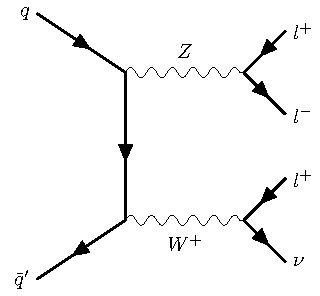
\includegraphics[width=\textwidth]{Feynman_WZ.pdf}
    \caption{}
    \label{fig:VVfeyna}
  \end{subfigure}
  \begin{subfigure}{0.45\figwidth}
    \centering
    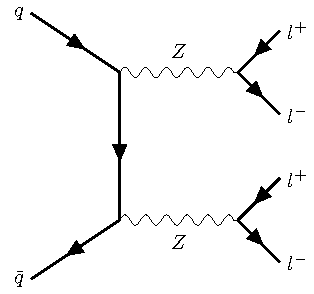
\includegraphics[width=\textwidth]{Feynman_ZZ.pdf}
    \caption{}
    \label{fig:VVfeynb}
  \end{subfigure}
  \caption[Feynman diagrams for \diboson backgrounds]{Feynman diagrams for the \diboson background}
  \label{fig:VVfeyn}
  \end{figure}

The \Ptop-quark pair production in association with a heavy boson (\PZ or \PW) can be an
important source of background. In particular, the \ttZ process, where the 
final state already includes a \PZ boson and a \Ptop quark, can produce a very 
similar signal-like signature. It is shown in \cref{fig:ttZ}. The \ttH contributes
less because of its small cross-section.

\begin{figure}
  \centering
      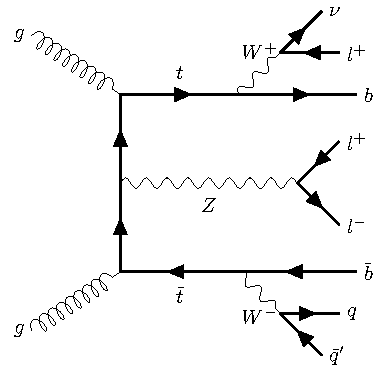
\includegraphics[width=0.45\textwidth]{Feynman_ttbarV.pdf}
      \caption{Feynman diagrams for the \ttZ background}
         \label{fig:ttZ}
\end{figure}

\subsection*{Backgrounds involving non-prompt leptons}

Backgrounds involving non-prompt or fake lepton are \Ptop-quark pair production 
and the production \PZ-boson with jets. 
As shown in \cref{fig:fakefeynb}, there are already two leptons
from the \PZ-boson. If the jets are light, they can be misidentified as leptons leading to 
a non-prompt lepton contribution.
In the \Ptop{}\APtop production, as shown in \cref{fig:fakefeynb}, if one of the \Pbottom-jet decays 
into a lepton, then it can satisfy the signal event selection.


\begin{figure}[htbp]
  \centering
  \begin{subfigure}{0.45\figwidth}
    \centering
    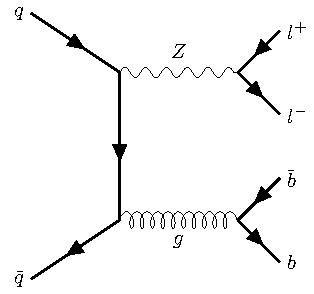
\includegraphics[width=\textwidth]{ZPlusJets_standalone.pdf}
    \caption{}
    \label{fig:fakefeyna}
  \end{subfigure}
  \begin{subfigure}{0.45\figwidth}
    \centering
    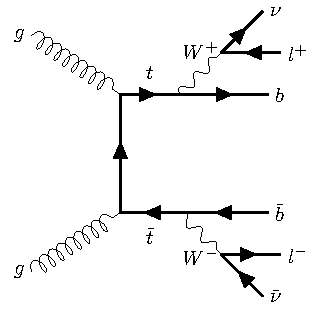
\includegraphics[width=\textwidth]{ttbar_standalone.pdf}
    \caption{}
    \label{fig:fakefeynb}
  \end{subfigure}
  \caption[Feynman diagrams for non-prompt lepton backgrounds]{Feynman diagrams for non-prompt lepton background}
  \label{fig:fakefeyn}
  \end{figure}

\section{Monte Carlo simulations and event generation}
\label{sec:MCinfo}

Monte Carlo simulations are a crucial part of this analysis, as they are used to interpret the detector data.. 
As already discussed before, proton-proton collisions are viewed as collisions between partons.
Given the number of incoming protons, fully understanding the collisions is complex. Moreover,
the randomness associated with it makes it difficult to use deterministic methods. Here is where, 
Monte Carlo (MC) simulations come to the rescue. MC simulation is a computational technique
to model a complex system using random numbers and underlying probability distribution functions.
In general, MC simulations use random numbers to sample from the underlying probability distribution
functions and then average the result of several iterations of sampling.  

In high energy physics, MC simulations are performed by MC generators which are also called event
generators. An event consists of a number of outgoing particles produced in accordance with 
conservation laws. However, quantum processes are inherently random and therefore, the outgoing 
particles vary from event to event. The task of an event generator is to generate random sequences 
of events based on given probability distribution functions. This task is not trivial because the 
structure of an event in hadron collisions is complex. Information about scattering, decays, 
radiations is required in order to accurately model an event. 
There is no comprehensive theory that can completely predict the properties of events. Thus, MC 
generators draw on theoretical models, with the Standard Model as their foundation, while also 
incorporating aspects derived from experimental data. In analyses, it is advised to test more 
than one generator because the extent of event modeling might be different for different generators. 

The resulting information from an event generator consists of four-momenta of stable particles, 
known as final state particles. Another use-case of MC generators is detector simulation where 
the evolution of the final state particles when they travel through the detector is simulated~\cite{mcgen}.  

The simulated data provided by these generators can be thought of as a "digital twin"
of the actual observed data. It can be used to predict any experimental observable or a combination of observables.
The workflow of MC generators, called as the MC chain, is a step-by-step process that begins with identifying the hard interaction and 
continues until the final state is achieved. At each stage, the structure of the underlying event 
evolves. The steps are briefly summarised below:

\begin{itemize}
  \item \textbf{Hard process}: In this step the hard process, defined as the process with the highest
  momentum transfer, is determined using matrix element calculation combined with the input Parton
  Distribution Functions. If a resonance is produced in a hard process, such as the \Ptop or \PZ and it
  shortly decays, then its decay process is also considered within the hard process. 

  \item \textbf{Parton Shower (PS)}: The colliding partons are responsible for emissions that give rise
  to more partons and subsequently more interactions. The emissions associated with the incoming partons
  is called Initial-State Radiation (ISR) while the emissions associated with the outgoing partons is called
  Final-State Radiation (FSR). These emissions and their respective interactions are modelled with
  Parton Shower algorithms. The incorporation of PS into the matrix element paints a more accurate picture
  of the collision process.

  \item \textbf{Multiple-processes}: Until now, only one of the partons from the original hadron is 
  considered but in reality, other partons from the same hadron also interact. Their interactions are
  termed as multiple-processes. They are calculated at this step of the MC simulation chain.
  
  \item \textbf{Hadronisation and decay}: The outgoing partons, with sufficient energy, can produce 
  new hadrons due to QCD colour confinement (hadronisation). If these hadrons are unstable, they can also
  decay into lighter particles. The MC chain also includes these calculations.
\end{itemize}

The MC chain results in a set of events with well-defined and stable final state particles along
with their kinematic distributions. At this stage, the simulated data is referred to as the 
\textit{truth-level} data. The next step is detector simulation where the interplay between the
detector material and final state particles is simulated. 

\mynote[inline]{}{Write details about detector response}

After all the MC events are generated, the interactions of the particles with the detector material is
simulated using the \textsc{GEANT4} software toolkit~\cite{Agostinelli:2002hh}.
Finally, the simulated data is ready for comparison with the observed detector data. The workflow of 
the MC chain is illustrated in \cref{fig:MCchain}.
Among the various available MC generators, \textsc{Herwig}~\cite{Bellm:2015jjp} and 
\textsc{Pythia}~\cite{Sjostrand:2007gs} are two of the most commonly used ones.

\begin{figure}
  \centering
      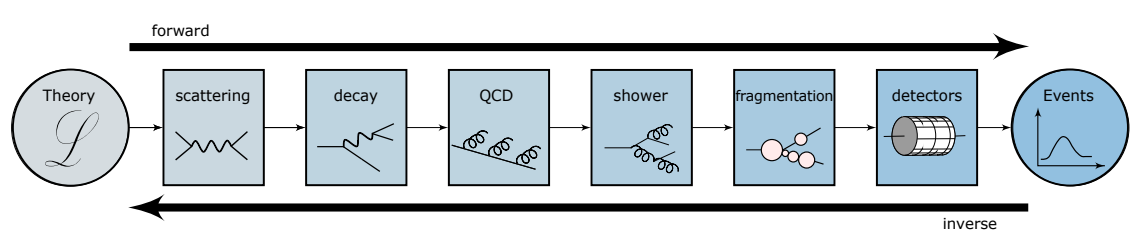
\includegraphics[width=0.8\textwidth]{MCchain.png}
      \caption{An illustration of the steps involved in a Monte Carlo chain~\cite{Plehn:2022ftl}}
         \label{fig:MCchain}
\end{figure}

\section{Data and simulated samples}
This analysis uses collision data collected by the ATLAS detector during 2015 to 2018 (Run-2 of the LHC) at a center of
mass energy of \qty{13}{\GeV}. The total integrated luminosity is of \lumi.

The ATLAS MC samples for analysis of the Run-2 dataset are divided into three subsets: 
\texttt{mc16a} generated with 2015 an 2016 pileup conditions, \texttt{mc16d} generated with 
2017 pileup conditions and \texttt{mc16e} that includes pileup conditions of 2018 data. 

\subsection{Signal sample}
The \tZq signal sample is simulated using \textsc{MadGraph5\_aMC@NLO} 2.9.5 generated at next-to-leading
order (NLO) with \textsc{NNPDF3.0NLO} parton distribution function. In general, the models used for
PS and hadronisation contain several free parameters which must be optimised to generate a reasonable
description of data. The optimisation is termed as tuning and the resulting sets of parameters are called
tune sets. For the signal sample, \textsc{Pythia} 8.245 is used for Parton Shower and
hadronisation along with A14 (ATLAS 24~\cite{ATL-PHYS-PUB-2014-021}) tune set and the \textsc{NNPDF2.3LO} PDF set.
The \Ptop-quark is decayed at LO using \textsc{MADSPIN}.
\mynote[inline]{}{UPDATE THIS AFTER NEW SAMPLE and add info about scales}

\subsection{Background samples}
For the background processes, different versions of \textsc{MadGraph5\_aMC@NLO}~\cite{Alwall:2014hca}, 
\textsc{Sherpa}~\cite{Gleisberg:2008ta} or \textsc{Powheg}~\cite{Banfi:2023mhz} generators are used to
calculate the matrix element and cross-sections combined with the \textsc{NNPDFx.xNLO} PDF set.
The PS and hadronisation is modeled with \textsc{Pythia} for the nominal background samples
and \textsc{Herwig} for the alternate sample generation. The alternate samples are required
for the theoretical uncertainties as described in SECTION. The specific versions
used for different backgrounds is summarised in \cref{tab:bkgmc}.

\mynote[inline]{}{Add the detailed DSIDs and everything in the appendix and refer here}

\begin{table}[htbp]
  \tablesetup
  \centering
  \caption{Background sample details} 
  \begin{tabular}{ l | l | l | l | l }
  \toprule
  Background & Generator &  Parton Shower &  PDF & Type of Sample \\
  \midrule
  \ttZ & \textsc{MadGraph5\_aMC@NLO} 2.8.1 & \textsc{Pythia} 8.244 & \textsc{NNPDF3.0NLO} & Nominal \\
  & & & \textsc{NNPDF2.3LO} & \\
  \ttZ & \textsc{MadGraph5\_aMC@NLO} 2.8.1 & \textsc{Herwig} 7.2.1 & \textsc{NNPDF3.0NLO} & Alternate \\
  & & & \textsc{NNPDF2.3LO} & \\
  \tWZ & \textsc{MadGraph5\_aMC@NLO} 2.X.X & \textsc{Pythia} 8.235 & \textsc{NNPDF3.0NLO} & Nominal \\
  \Diboson & \textsc{Sherpa} 2.2.12 & \textsc{Sherpa} \textsc{MEPS@NLO} & \textsc{NNPDF3.0NNLO} & Nominal \\
  \Triboson & \textsc{Sherpa} 2.2.2 & \textsc{Sherpa} \textsc{MEPS@NLO} & \textsc{NNPDF3.0NNLO} & Nominal \\
  \ttbar & \textsc{Powheg Box v2} & \textsc{Pythia} 8.230 & \textsc{NNPDF3.0NLO} & Nominal \\
  & & & \textsc{NNPDF2.3LO} & \\
  \ttbar & \textsc{Herwig} 7.2.1 & \textsc{Pythia} 8.230 & \textsc{NNPDF3.0NLO} & Alternate \\
  \tW & \textsc{Powheg Box v2} & \textsc{Pythia} 8.230 & \textsc{NNPDF3.0NLO} & Nominal \\
  & & & \textsc{NNPDF2.3LO} & \\
  \Zjets & \textsc{Sherpa} 2.2.11 & \textsc{Sherpa} \textsc{MEPS@NLO} & \textsc{NNPDF3.0NNLO} & Nominal \\
  \ttW & \textsc{Sherpa} 2.2.10 & \textsc{Sherpa} \textsc{MEPS@NLO} & & Nominal \\
  \ttH & \textsc{Powheg Box v2} & \textsc{Pythia} 8.230 & \textsc{NNPDF3.0NLO} & Nominal \\
  & & & \textsc{NNPDF2.3LO} & \\
  \ttt & \textsc{MadGraph5\_aMC@NLO} 2.2.2 & \textsc{Pythia} 8.186 & \textsc{NNPDF2.3LO} & Nominal \\
  \tttt & \textsc{MadGraph5\_aMC@NLO} 2.3.3 & \textsc{Pythia} 8.230 & \textsc{NNPDF3.1LO} & Nominal \\
  \tttt & \textsc{MadGraph5\_aMC@NLO} 2.3.3 & \textsc{Herwig} 7.0.4 & \textsc{NNPDF3.1LO} & Alternate \\
  \bottomrule
  \end{tabular}
  \label{tab:bkgmc}
  \end{table}

\section{Systematic Uncertainties}
\label{sec:systinfo}
One of the key advantages of using simulated data is their ability to predict how the observed data may appear. 
However, it is crucial to assess how dependable both the simulated and the measured data are, which
is quantified through uncertainties. The proper inclusion of uncertainties is an important part of any analysis.

Uncertainties can be divided into two sections: statistical and systematic. Simply put, statistical uncertainties are
related to the statistics of the data whereas systematic uncertainties are complex uncertainties 
that are not directly from the statistics of the data. For instance, the length of an object is measured with a 
ruler and is found to be $10 \pm 0.5$ cm. Here the statistical uncertainty is $0.5$ cm. In addition,
there is a systematic uncertainty which can originate from the calibration of the ruler. 

In high energy physics, sources of systematic uncertainties are calibrations of scales, efficiencies of 
particle identifications and reconstructions, choice of MC generators, etc. These sources of systematic
uncertainties are categorised into: instrumental and theoretical uncertainties as described
in \cref{sec:systdescribe} and \cref{sec:systdescribe2}, respectively. 

\subsection{Instrumental or detector uncertainties}
\label{sec:systdescribe}

\begin{itemize}
  \item \textbf{Luminosity}: The integrated luminosity is \lumi and the uncertainty in its calculation
  is $0.83\%$

  \item \textbf{Pileup reweighting}: MC generators make use of scale factors to account for differences in 
  pileup distributions between data and simulations. There is an uncertainty associated with these 
  scale factors. It is evaluated by changing the nominal pileup value to a lower and a higher value,
  then the effect of these changes is calculated to obtain the up and down uncertainty.

  \item \textbf{Jet Energy Scale (JES)}: After the jets are reconstructed, their energies need to be 
  adjusted so that it reflects the energy of the colliding particles. The calibration is done by 
  comparing the reconstructed jets with the true jets which are simulated jets of stable particles 
  without detector effects. Uncertainties originating from the calibration process are categorised 
  as JES uncertainties~\cite{Barillari2012}.

  \item \textbf{Jet Energy Resolution (JER)}: JER is the detector's ability to distinguish two jets 
  with similar total energy. The uncertainty associated with the differences in JER in case of data and 
  simulation is called JER uncertainty. 

  \item \textbf{Jet-Vertex-Tagger (JVT)}: It is a discriminant in the form of likelihood constructed 
  using track-based variables, sensitive to the origin of jets. A cut is applied on the JVT factor to
  reject jets coming from pileup~\cite{ATL-PHYS-PUB-2015-040}. The uncertainty associated with the JVT factor 
  is one of the systematics.

  \item \textbf{Lepton reconstruction}: Scale factors are applied to correct differences between data and
  simulation in case of lepton identification, isolation and trigger efficiencies. The uncertainties
  associated with these scale factors belong to the lepton reconstruction category of systematics.  

\end{itemize}

\subsection{Theoretical uncertainties}
This category involves uncertainties originating from the various models used in the MC simulation 
chain, and therefore, also called modeling uncertainties or modeling systematics. There are various 
parameters related to the modelling of a certain process and for each parameter, there is 
an associated uncertainty which is investigated by varying the values of the parameters. The effect of 
the variation is estimated and assigned as the systematic uncertainty. In this way,
the uncertainties associated with the modelling of the process is extracted. 
  
\begin{itemize}
  
  \item \textbf{A14}: The uncertainty associated with the A14 tune set is determined by comparing the nominal sample with 
  two alternate samples, both simulated using the same settings as the nominal sample but incorporating 
  the up and down variations of the A14 tune set. This variation is related to the strong 
  coupling constant $\alpha_s$. This uncertainty is considered for \tZq and \ttZ processes. 

  \item \textbf{Scale}: The parameters representing renormalisation and factorisation scales are 
  known as $\mu_R$ and $\mu_F$, respectively and their values are $\mu_R$=$\mu_F$=$H_T/6$. The renormalisation
  scale is for the running of $\alpha_S$ associated with the hard process whereas the 
  factorisation scale for the PDFs. They are introduced to prevent the matrix 
  element from any possible divergences. In order to estimate the uncertainty on the parameters, the values
  of $\mu_R$ and $\mu_F$ are varied between $\mu_R$=$\mu_F$=0.5, $\mu_R$=$\mu_F$=1 and $\mu_R$=$\mu_F$=2. This
  uncertainty is considered for \tZq, \diboson and \ttZ processes.

  \item \textbf{Shower and PDF}: The showering uncertainty is calculated by comparing the nominal sample (modeled using \textsc{Pythia})
  and the alternate sample (modeled using \textsc{Herwig}). Moreover, uncertainty associated 
  with the \mynote{PDF}{write about pdf4lhc} is also considered. The shower systematic is included for \tZq, \ttZ and \ttbar processes
  whereas the PDF uncertainty is considered for \tZq, \diboson and \ttZ processes. 

  \item \textbf{Interference}: This uncertainty accounts for the interference between \ttZ and \tWZ
  processes. The non-resonant \tWZ production can feature a resonant $\APtop$ in the intermediate state,
  leading to overlap with the \ttZ production. This interference is navigated using various techniques 
  called diagram removal (DR) and diagram subtraction (DS). Two \tWZ samples were generated, one with 
  DR1 and another with DR2 and the difference is taken to be the \tWZ modeling uncertainty. 

  \item \textbf{Matrix element matching and resummation}: The systematics in this category are
  taken into account for the \diboson process following the recommendations
  of the Physics Modelling Group~\cite{twikiPMG,twikiPMGVV}. The CKKW parameter is related to the calculation of 
  the overlap between jets involved in the matrix element and parton shower computation. The nominal 
  value of the parameter CKKW is \qty{20}{GeV} and its uncertainty is estimated by varying this value 
  to \qty{30}{GeV} (up variation) and \qty{15}{GeV} (down variation)~\cite{Anders:2125718}. The QSF parameter determines the 
  scale for the resummation of soft gluon emissions. Its uncertainty is estimated by varying the nominal
  by 2 and 0.5~\cite{Anders:2125718}.

  In the parton shower computation, a recoil scheme refers to how the remaining partons adjust their
  momenta after emission or splitting, in order to conserve the total momentum. The recoil scheme used
  for the \diboson samples is described in~\cite{Schumann:2007mg}. The uncertainty on the associated parameter CSSKIN is 
  also considered for the \diboson process. Finally, approximate NLO EW corrections are included as weights using
  the electroweak virtual approximation as described in~\cite{Kallweit:2014xda}. 

  \item \textbf{Matching and ISR}: The \ttbar background is being modelled using \textsc{Powheg}
  generator in which a parameter called $h_{\text{damp}}$ is the damping factor that controls the radiation
  at which the \ttbar system recoils. If this is set to infinity then all the radiation is considered
  in the computation of ISR. The uncertainty on ISR is estimated by comparing two nominal \ttbar 
  samples, one with $h_{\text{damp}}$=$1.5m_t$ and second with $h_{\text{damp}}$=$3m_t$.

  Depending on the generator and parton shower workflow, there might be overlapping phase spaces
  which can cause double-counting of events. To prevent this, a parameter called \textsc{pThard} is defined 
  which refers to the hard scattering transverse momentum scale. This parameter decides the extent of 
  phase space which is vetoed while matching matrix element with the parton shower. 
  The uncertainty on \textsc{pThard} is estimated
  by comparing samples with \textsc{pThard}=1 and \textsc{pThard}=0.
\end{itemize}
\label{sec:systdescribe2}

\section{Event weights}

The collision events generated from the MC simulations must be reweighted in order to reproduce
data-taking conditions. The probability of
an event, relative to the sum of probabilities for the sample, is given by its MC event weight ($w_{\text{MC}}$).
The MC event weights are important because the sum of these weights will determine the 
correct number of events for that sample. 

% The events generated from the Monte Carlo simulation are unweighted, which means that each event 
% represents an equal share of the total cross-section. However, for obtaining a correct distribution
% of an observable, each raw event is required to be weighted. Generally, these weights are provided by the
% MC generator.

In addition, a number of correction factors are applied in order to match the data-taking conditions
as well as correcting differences in efficiencies of identifying physics objects. Some weights also correspond to a 
systematic variation. Consider a systematic which 
requires a parameter to be varied. Now, producing the entire event sample with the varied 
parameter is computationally intensive. Instead, a corresponding weight is included in the event 
generation~\cite{10.21468/SciPostPhysCodeb.8}.

The total event weight can be written as:

\begin{equation}
  w_{\text{total}} = w_{\text{MC}} \cdot w_{\text{pileup}} \cdot w_{\text{lepton}} \cdot w_{\text{JVT}} \cdot w_{\text{trigger}} \cdot w_{\text{\Pbottom-tagging}}
\end{equation}


\begin{itemize}
  \item $w_{\text{MC}}$: gives the relative probability of producing that event in that sample
  \item $w_\text{pileup}$: to correct the pileup profile of simulated events to match observed data
  \item $w_{\text{lepton}}$: to correct for the differences in lepton isolation and reconstruction between
  MC and data
  \item $w_{\text{JVT}}$: differences in data and MC when applying a cut on the JVT factor are considered
  by applying this weight
  \item $w_\text{trigger}$: any inconsistency between data and MC related to trigger efficiencies is
  corrected with this weight
  \item $w_\text{\Pbottom-tagging}$: this analysis requires events to contain \Pbottom-jets. This is 
  ensured by a applying a weight called $w_\text{\Pbottom-tagging}$
\end{itemize}


\section{Artificial Neural Networks}
A neural network is a computation tool developed to function in a way similar to the human mind. It is 
widely used in high energy physics for data analysis. The structure of a neural network (NN) is made 
up of neurons or \textit{nodes}. Their function is to examine unknown systems and identifying 
interesting features, just like the job of neurons in human mind. Generally, these nodes are arranged 
in three different layers: the input layer, the hidden layer and the output layer. A list of variables 
is given as input to the nodes of the input layer. Processing takes place through the subsequent 
layers and at the end, the output layer returns the conclusions derived by the network. Connections 
between nodes of different layers are referred to as the \textit{synapses}. Each connection between 
nodes of two consecutive layers, has a weight associated to it. \Cref{fig:NN} shows a diagram of a neural network. 

\begin{figure}[htbp]
  \centering
    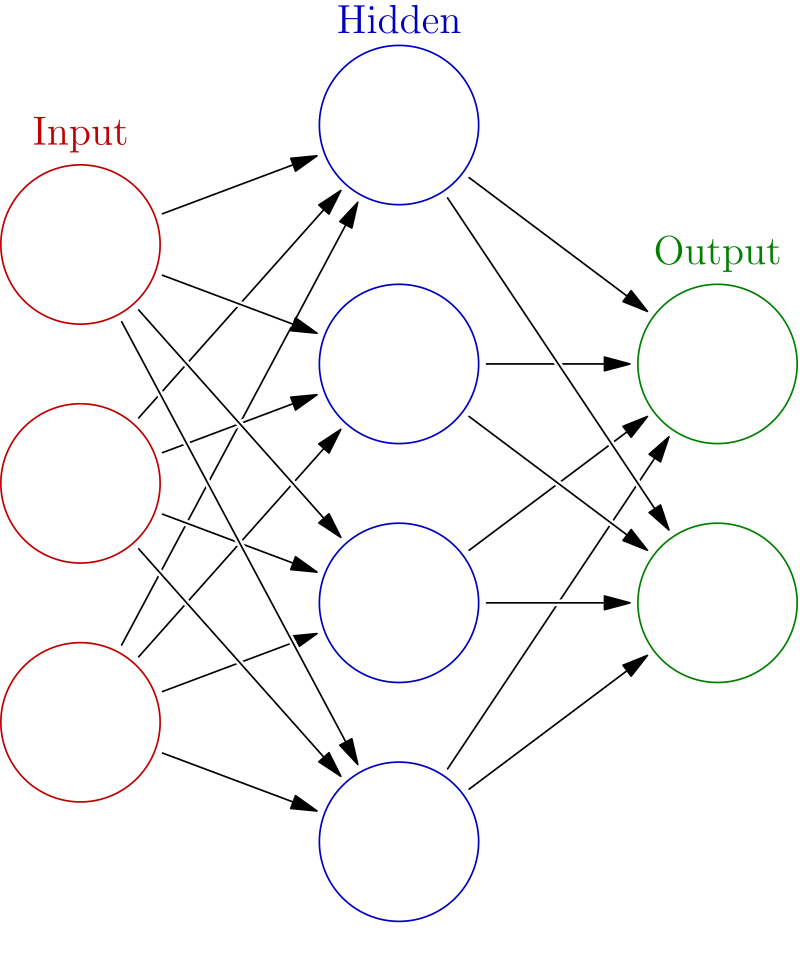
\includegraphics[width=0.7\figwidth]{NN.png}
  \caption[Neural Network]{Diagram of a neural network including the input, hidden and output 
  layers~\cite{NN}}
  \label{fig:NN}
\end{figure}

The input received by each node is the sum of weighted output of all nodes of the previous layer. 
As given in Equation~\ref{eqn:4.2}, $y_j$ is the input to node $j$, $w_{ij}$ is the weight from the 
$i$-th node and $x_i$ is that node's output. The term $w_{0j}$ is called bias. 

\begin{equation}
    y_j = \Sigma_{i=1}^{n} w_{ij}x_i + w_{0j} 
    \label{eqn:4.2}
\end{equation}


The output of a node is defined by an \textit{activation} function. Common choice of an activation 
function is the sigmoid function. It provides output between 0 and 1. A feature that makes a NN special
is its capability to \textit{learn} from examples with known inputs and outputs. This is referred to 
as \textit{training} a neural network. The purpose of training is to find appropriate weights. 
In supervised training, inputs and outputs are provided to a NN. It processes input and then compares 
the resultant output with the desired output. Comparison is done by calculating 
a \textit{loss function}. It is a way to determine how well is the network trained. For better
performance of a network the loss function should be minimised. In order to do that, errors of the 
resultant output are propagated back in a model and the initial weights are readjusted so that 
output is closer to the desired output. This is how a network learns. A dataset flows inside a 
network several times and each time weights are refined until a minimum value of the loss function 
is obtained.
